% Chapter Template

\chapter{Long Short-Term Memory} % Main chapter title

\label{Chapter4} % Change X to a consecutive number; for referencing this chapter elsewhere, use \ref{ChapterX}

%----------------------------------------------------------------------------------------
%	SECTION 1
%----------------------------------------------------------------------------------------

\section{Understanding LSTMs}

Long Short Term Memory networks – usually just called \textit{LSTMs} – are a special kind of RNN, capable of learning long-term dependencies. They were introduced by Hochreiter and Schmidhuber (1997).

LSTMs are explicitly designed to avoid the long-term dependency problem. This allows the network to remember information for long periods of time.

All recurrent neural networks have the form of a chain of repeating modules of neural network. But the core of the LSTMs is the \textit{cell state}, that allows the network to keep a simple state information through the processing of all the time steps in the chain. An scheme of a LSTM architecture is described in figure \ref{fig:lstm}.

\begin{figure}
%\centering
\begin{center}
  \makebox[\textwidth]{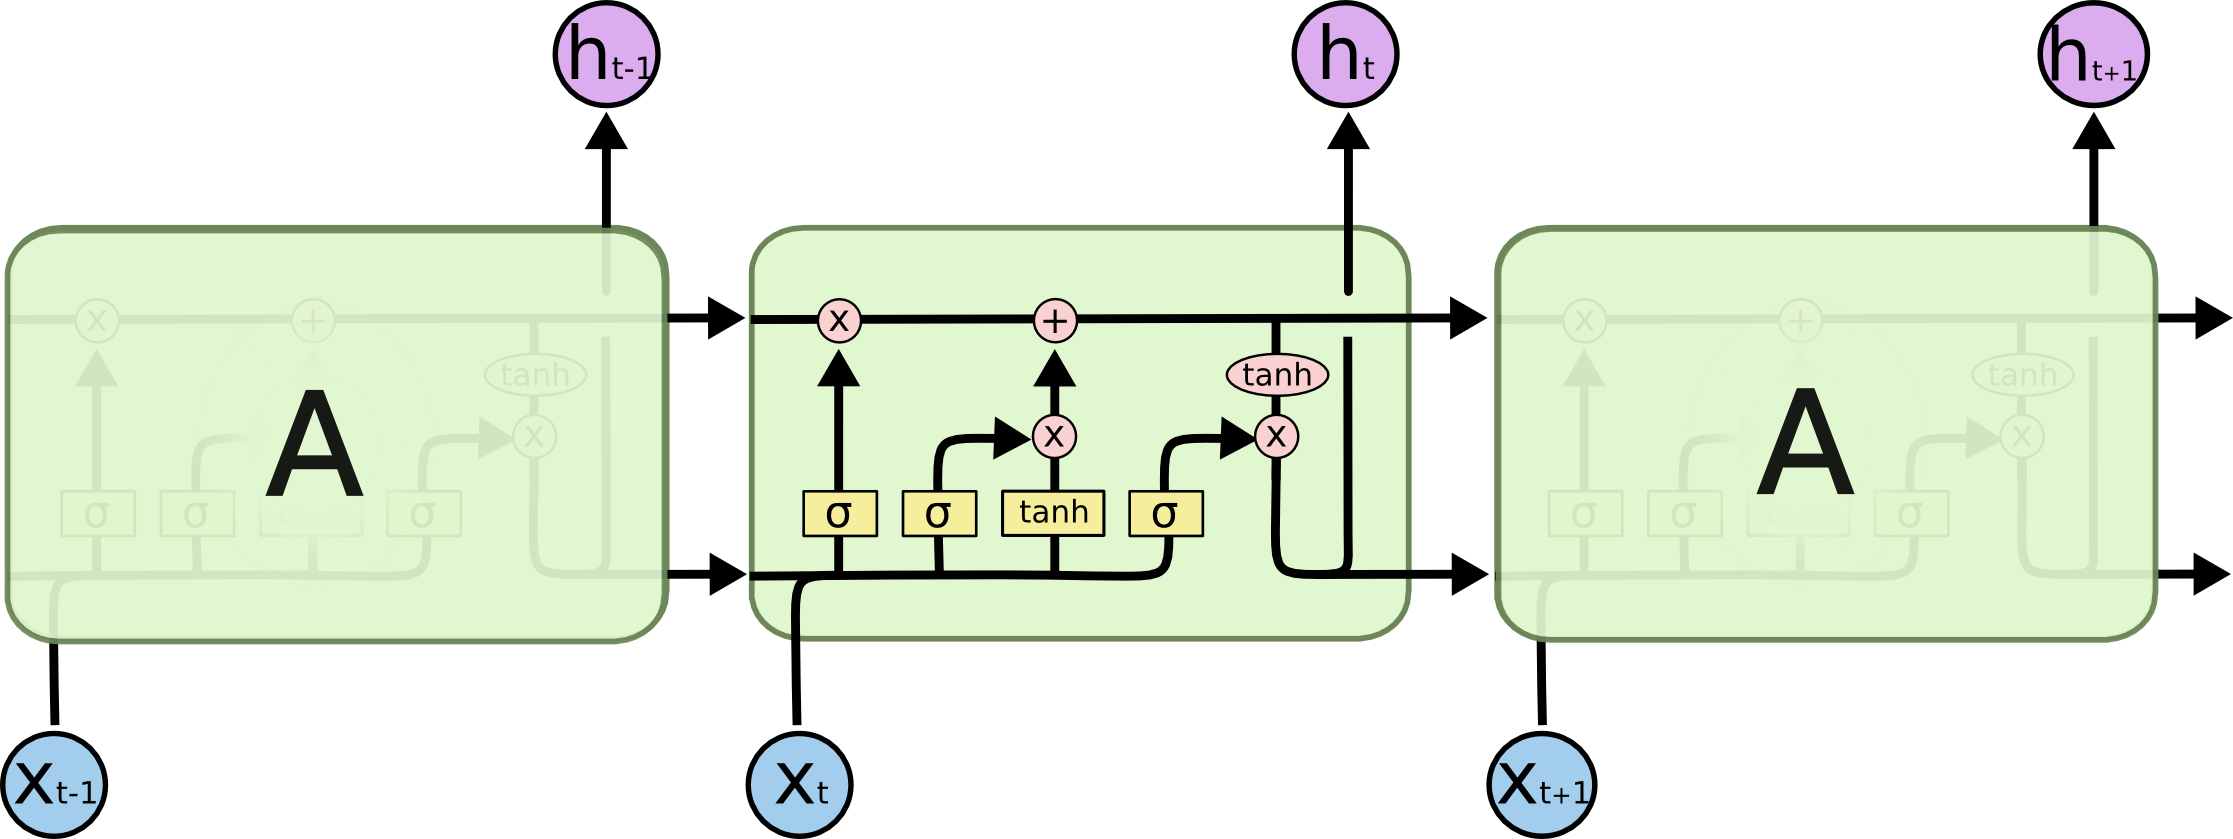
\includegraphics[width=\textwidth]{Figures/LSTM}}
\end{center}
\decoRule
\caption[LSTM architecture]{LSTM architecture.}
\label{fig:lstm}
\end{figure}

\section{Binary Classification}

The next sections describe the methodology applied to solve the binary classification problem using LSTMs

%-----------------------------------
%	SUBSECTION 1
%-----------------------------------
\subsection{Data Generation}

Before the ingestion of the data into the LSTM model, it has to be adapted to the architecture of the network.

Being \textit{samples} the total number of data, \textit{timesteps} the amount of rows to be ingested for each aircraft and \textit{features} the number of sensor data the input of the LSTM layer is defined by a tensor of shape:

\begin{verbatim}
    (samples, timesteps, features)
\end{verbatim}

The time steps used for the study will be 50, which means that for each aircraft batches of 50 time steps will be taken.
Using the \textit{zip} function over the data of the aircraft with id=1, which contains 192 cycles. The batches will be distributed this way:

\begin{verbatim}
    (0, 50)     -> from row 0 to row 50
    (1, 51)     -> from row 1 to row 51
    (2, 52)     -> from row 2 to row 52
    ...
    (111, 192)  -> from row 111 to row 192
\end{verbatim}

After the pre-processing, the input tensor will have the shape:

\begin{verbatim}
    (15631, 50, 25)
\end{verbatim}

To generate the labels the values of the column \textit{label 1}, which was generated on the data preparation (see chapter \ref{Chapter3}), must be grouped by aircraft indicating if the engine failed within \textit{w1} cycles.

The result label tensor has the shape:

\begin{verbatim}
    (15631, 1)
\end{verbatim}

%-----------------------------------
%	SUBSECTION 2
%-----------------------------------

\subsection{Model definition}

Work in progress...